\documentclass[12pt]{article}
   
\usepackage[utf8]{inputenc}
   \usepackage{graphicx}
   \usepackage{float}
   \usepackage{subcaption}
   %\usepackage{mathtools}
   \usepackage{amsmath}
   \usepackage{listings}
    \usepackage{xcolor}
    
    \definecolor{codegreen}{rgb}{0,0.6,0}
    \definecolor{codegray}{rgb}{0.5,0.5,0.5}
    \definecolor{codepurple}{rgb}{0.58,0,0.82}
    \definecolor{backcolour}{rgb}{0.95,0.95,0.92}
    
    \lstdefinestyle{codestyle}{
        backgroundcolor=\color{backcolour},   
        commentstyle=\color{codegreen},
        keywordstyle=\color{magenta},
        numberstyle=\tiny\color{codegray},
        stringstyle=\color{codepurple},
        basicstyle=\ttfamily\footnotesize,
        breakatwhitespace=false,         
        breaklines=true,                 
        captionpos=b,                    
        keepspaces=true,                 
        numbers=left,                    
        numbersep=5pt,                  
        showspaces=false,                
        showstringspaces=false,
        showtabs=false,                  
        tabsize=2
    }
    
    \lstset{style=codestyle}

   \addtolength{\hoffset}{-0.7in}
   \addtolength{\textheight}{1.5in}
   \addtolength{\textwidth}{1.5in}
   \addtolength{\voffset}{-1in}
%
% Title.
\title{EE230: Experiment 6\\
Phase Sensitive Detection (Lock-in-amplifier)}

% Author
\author{Hitesh Kandala, 180070023}

% begin the document.
\begin{document}

% make a title page.
\maketitle
\tableofcontents
\clearpage

\section{Overview of the experiment}

    \subsection{Aim of the experiment}
        In this experiment, we construct a lock-in-amplifier using the following blocks that it comprises of -
        \begin{enumerate}
            \item Buffer(Voltage Follower)
            \item Phase Shifter
            \item Switch Driving Circuit
            \item Switch based Phase Sensitive Detector
            \item Low Pass Filter
        \end{enumerate}
%%%%%%%%%%%%%%%%%%%%%%%%%%%%%%%%%%%%%%%%%%%%%%%%%%%%%%%%%%%%%%%%%%%%%%%%%%%%%%%%%%%%%%%%%%%%%%%%%
    \subsection{Theory}
        The lock-in-amplifier is comprises of five blocks of circuit implementation as shown below:
        \begin{figure}[H]
            \centering
            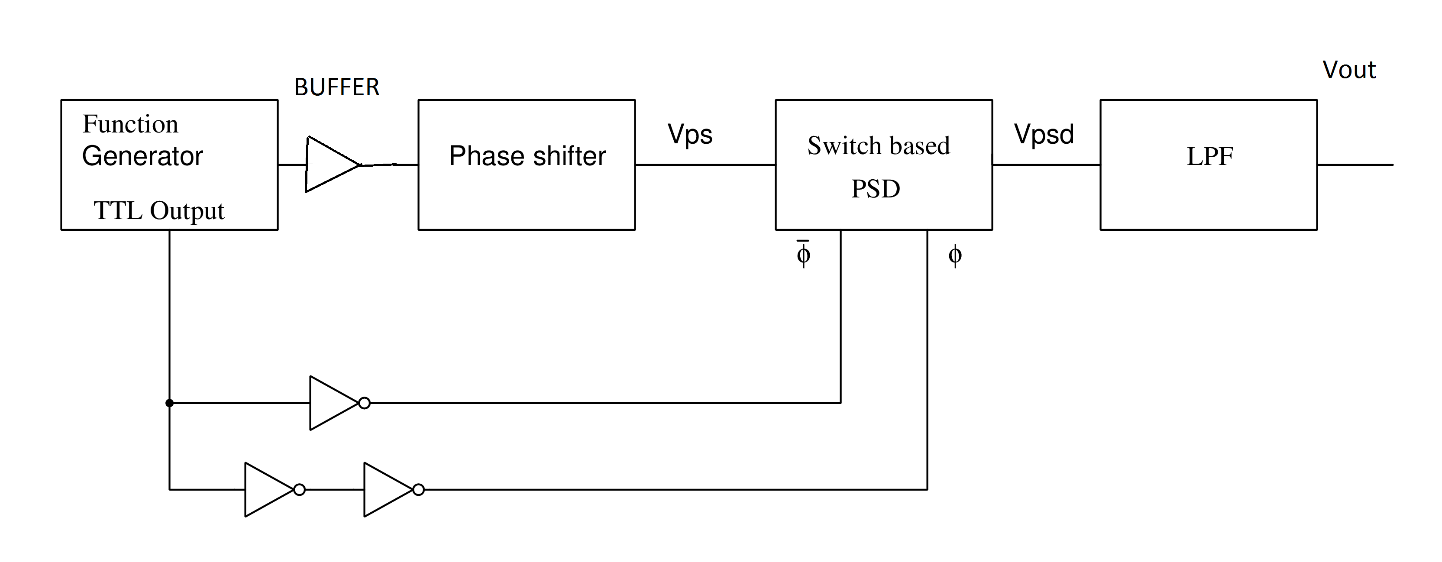
\includegraphics[width=0.6\linewidth]{reports/lab6/block.png}
            \caption{Block diagram of PSD}
            \label{fig:instru}
        \end{figure}
        
        \subsubsection{Buffer: 741 based voltage follower}
            The Op-Amp Buffer is a non inverting amplifier, with gain exactly \textbf{1}. It is also known as Voltage Follower since the output voltage exactly mirrors the input voltage.\\\\
            Buffer circuit prevents loading of the source. If the load to a voltage source is a low value, it practically shorts the source and draws too much current from the source for which the source is not rated which is harmful for the source. So by cascading a buffer after a source provides division of labour - the source only generated the correct voltage and the buffer provides the demanded current keeping the voltage constant and without loading the source as the buffer has very high input impedance, it draws negligible current from the original source, thereby preventing loading.
        
        \subsubsection{Phase Shifter}
            Phase shifter is simply used to get two square waves complementary to each other. This is achieved using CMOS inverters.
            
        \subsubsection{Switch Driving Circuit}
            This circuit is used to produce two complimentary square wave signals of a 5V amplitude using IC 74C04 (CMOS inverters). These signals are required to drive two pairs of analog switches in phase sensitive detector as control inputs.  
            
        \subsubsection{Switch based phase sensitive detector}
            \begin{figure}[H]
                \centering
                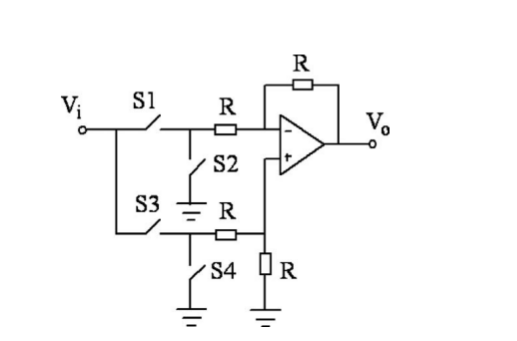
\includegraphics[width = 0.5\linewidth]{reports/lab6/manualswitch.png}
                \caption{Analog switches}
            \end{figure}
            \noindent
            It consists of an op-amp, which is configured as a differential amplifier, and four single-pole single-throw (SPST) analog switches, which are controlled by two complementary square waves.
            \begin{figure}[H]
                \centering
                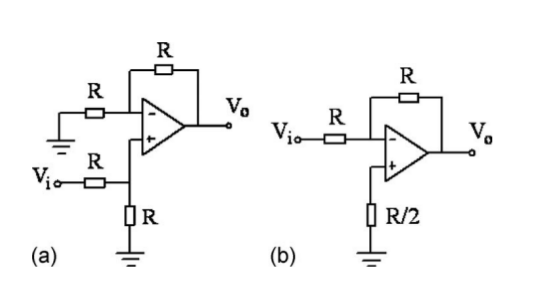
\includegraphics[width = 0.5\linewidth]{reports/lab6/equi.png}
                \caption{Equivalent circuit configurations}
            \end{figure}
            \noindent
            The circuit is operated in two phases. As indicated in Fig 2, in phase 1, switches S2 and S3 are ON and S1 and S4 are OFF. In this case the circuit in Fig. 2 is equivalent to a non-inverting amplifier with unit gain as shown in Fig. 3(a). In phase 2, S1 and S4 are ON and S2 and S3 are OFF. In this case the circuit in Fig. 2 is equivalent to an inverting amplifier also with unit gain as shown in Fig. 3(b). In other words, in phase 1 the gain of the circuit is 1 and in phase 2 the gain is -1.
            \\\\
            Let's assume the input signal is a sine wave,
            \begin{align}
                V_i = A sin(\omega t + \phi)
            \end{align}
            \noindent
            The switching function can be described by:
            \begin{align}
                gain &= 1 \qquad \, when \quad 0 < \omega t < \pi \\
                     &= -1 \qquad when \quad \pi < \omega t < 2\pi
            \end{align}
            \noindent
            so that
            \begin{align}
                V_o &= V_i = A sin(\omega t + \phi) \qquad \, when \quad 0 < \omega t < \pi \\
                     &= V_i = -A sin(\omega t + \phi) \qquad when \quad \pi < \omega t < 2\pi
            \end{align}
            
        \subsubsection{Low pass filter}
            The average output of the PSD circuit on calculating by integration comes out to be, 
            \begin{equation}
                \overline{\rm V} = \frac{2A}{\pi}cos\phi 
            \end{equation}
            The above equation represents the output of the PSD after the harmonics is removed by a low-pass filer with a sufficiently low cutoff frequency. This analytical result indicates that the output of the switch-based PSD unit is a function of not only the amplitude of the input sine-wave signal A, but also the phase difference $\phi$ between the input sine-wave signal and the reference square wave.
            

    \subsection{Apparatus Required}

        \begin{itemize}
            \item IC 741 \(\times\)4
            \item IC 74C04
            \item IC CD4066
            \item Arbitrary Function Generator
            \item Resistors: 10k\(\Omega\) \(\times\)6, 15k\(\Omega\) \(\times\)2, 10k\(\Omega\) Pot
            \item Capacitors: 1\(\mu\)F \(\times\)2
            \item Connecting Wires
            \item Breadboard \(\times\)2
            \item DMM and DSO
        \end{itemize}

 %%%%%%%%%%%%%%%%%%%%%%%%%%%%%%%%%%%%%%%%%%%%%%%%%%%%%%%%%%%%%%%%%%%%%%%%%%%%%%%%%%%%%%%%%%%%%%%%           
\section{Experimental results}
    
%%%%%%%%%%%%%%%%%%%%%%%%%%%%%%%%%%%%%%%%%%%%%%%%%%%%%%%%%%%%%%%%%%%%%%%%%%%%%%%%%%%%%%%%%%%%%%%%%%%%%%
    \subsection{Buffer using IC 741}
        \textbf{Observations and Inferences}\\
        
        The cicuit of buffer is as shown below:  
        \begin{figure}[H]
            \centering
            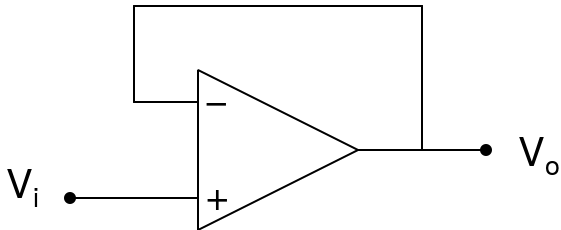
\includegraphics[width = 0.4\linewidth]{reports/lab6/buffer.png}
            \caption{Buffer Circuit}
        \end{figure}
        \noindent
        This is the first block and is connected to input voltage.\\\\
        The input voltage applied here is 1 $V_{pp}$, 1 KHz.

%%%%%%%%%%%%%%%%%%%%%%%%%%%%%%%%%%%%%%%%%%%%%%%%%%%%%%%%%%%%%%%%%%%%%%%%%%%%%%%%%%%%%%%%%%%%%%%%%%%%%%%%   
    \subsection{Phase Shifter}
        \noindent
        \textbf{Observations and Inferences}\\
        \noindent
        The circuit diagram of phase shifter is shown below.\\
        Here in the circuit $R3 = 10k$, $R4 = 10k$, $R1 = 10k$ pot and $C = 1\mu F$
        \begin{figure}[H]
            \centering
            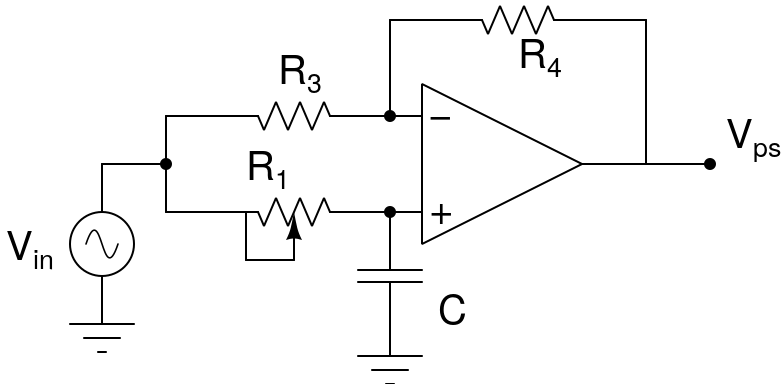
\includegraphics[width = 0.4\linewidth]{reports/lab6/phaseshifter.png}
            \caption{Circuit of wien bridge oscillator}
        \end{figure}
        \noindent
        The op-amp used in the above circuit is 741 and the ideal values of the passive elements used are $C = 1\mu F$, $R_3 =9.69k\Omega$, $R_4 = 9.76k\Omega$, $R_1 = 10k\Omega$ pot.\\
        \noindent
        The transfer function for this Phase Shifter is given by,
        \begin{equation}
            H(j\omega)=\frac{1-j\omega R \times 1\mu F}{1+j\omega R \times 1\mu F}
        \end{equation}
        \noindent
        The phase response of the Phase Shifter is given by,
        \begin{equation}
            \angle H(j\omega)=-2\arctan(\omega R \times 1\mu F)
        \end{equation}
        \noindent
        The magnitude response of the Phase Shifter is given by,
        \begin{equation}
            |H(j\omega)|=1
        \end{equation}
        Since, \(|\)H(j\(\omega\))\(|\) = 1 \forall \(\omega\), the Phase Shifter is also known as All Pass Filter.\\
        \noindent
        The observations of this part are in the table below. We tabulate both the Calculated and Observed values of Resistance for different values of phase shift in the table below.
        
        \begin{center}
            \begin{tabular}{|c|c|c|}
            \hline
            Phase Difference(^\circ)  &   Calculated Resistance(\(\Omega\)) &   Observed Resistance(\(\Omega\)) \\
            \hline
            0   &   0     &   0      \\
            -45   &   65.9 &   65     \\
            -90   &   159.2 &   155    \\
            -135   &   384.2 &   390    \\
            -180    &   \infty &   9270   \\
            \hline
            \end{tabular}
        \end{center}
        \noindent
        Some of the shifted waveforms are shown below:
        \begin{figure}[H]
            \centering
            \begin{subfigure}{.5\textwidth}
                \centering
                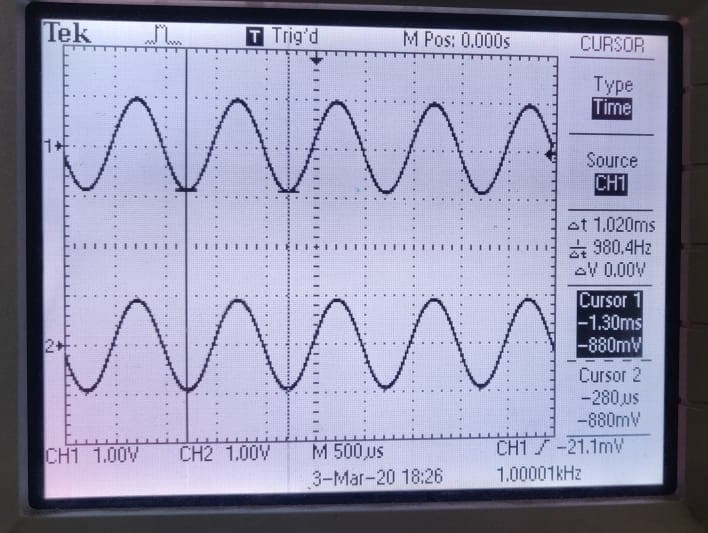
\includegraphics[width=70mm]{reports/lab6/phasediff.jpeg}
                \caption{Phase shift of 0}
            \end{subfigure}%
            \begin{subfigure}{.5\textwidth}
                \centering
                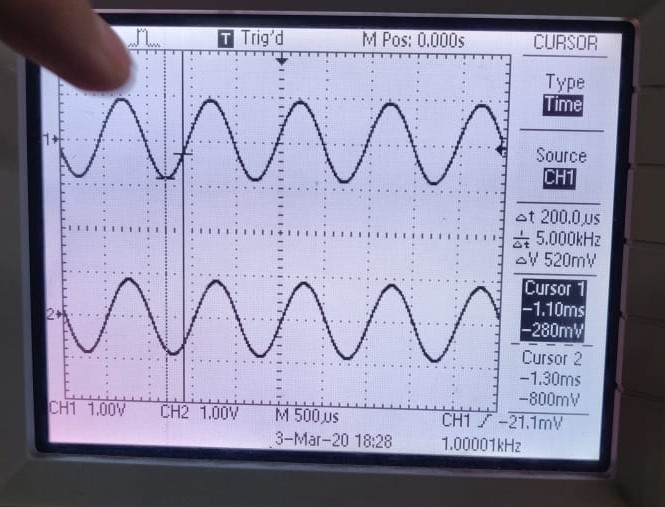
\includegraphics[width=70mm]{reports/lab6/phasediff2.jpeg}
                \caption{Phase shift of some \phi}
            \end{subfigure}%
        \end{figure}
        \noindent
        The phase response plotted on DSO is shown below:
        \begin{figure}[H]
            \centering
            \begin{subfigure}{.5\textwidth}
                \centering
                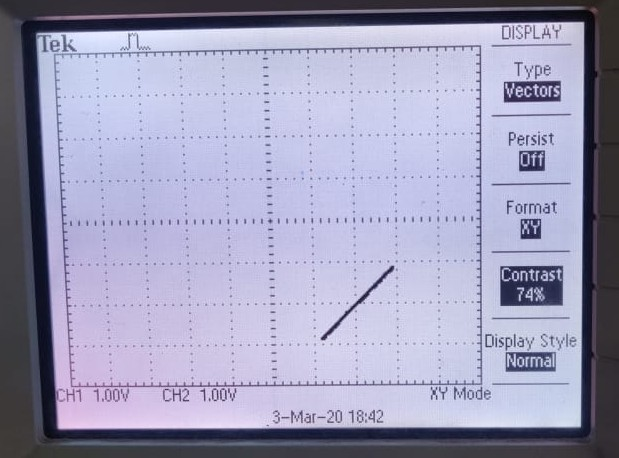
\includegraphics[width=70mm]{reports/lab6/first0.jpeg}
                \caption{$V_{out}$ vs $V_{in}$ for 0^{\circ}}
            \end{subfigure}%
            \begin{subfigure}{.5\textwidth}
                \centering
                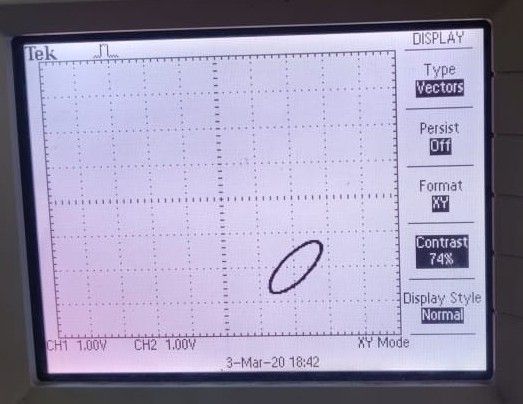
\includegraphics[width=70mm]{reports/lab6/first45.jpeg}
                \caption{$V_{out}$ vs $V_{in}$ for 45^{\circ}}
            \end{subfigure}%
        \end{figure}
        \begin{figure}[H]
            \centering
            \begin{subfigure}{.5\textwidth}
                \centering
                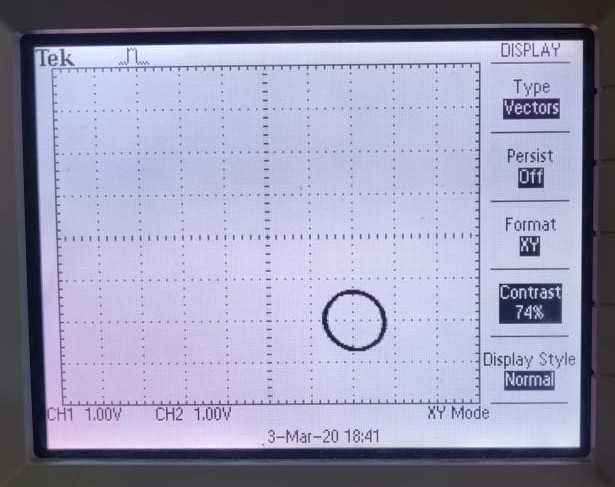
\includegraphics[width=70mm]{reports/lab6/first90.jpeg}
                \caption{$V_{out}$ vs $V_{in}$ for 90^{\circ}}
            \end{subfigure}%
            \begin{subfigure}{.5\textwidth}
                \centering
                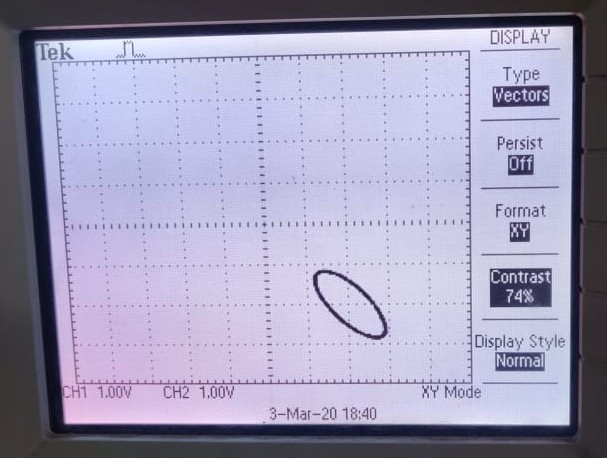
\includegraphics[width=70mm]{reports/lab6/first135.jpeg}
                \caption{$V_{out}$ vs $V_{in}$ for 135^{\circ}}
            \end{subfigure}%
        \end{figure}
        \begin{figure}[H]
            \centering
            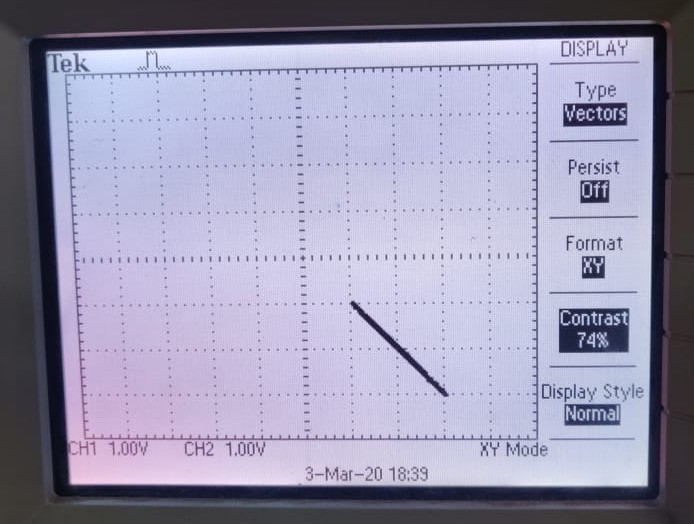
\includegraphics[width = 0.5\linewidth]{reports/lab6/first180.jpeg}
            \caption{$V_{out}$ vs $V_{in}$ for 180^{\circ}}
        \end{figure}
% "Insert the peak to peak voltage and frequency value as seen in the DSO pic"
%%%%%%%%%%%%%%%%%%%%%%%%%%%%%%%%%%%%%%%%%%%%%%%%%%%%%%%%%%%%%%%%%%%%%%%%%%%%%%%%%%%%%%%%%%%%%%%%%%%%%%%%%%   
    \newpage
    \subsection{Switch Driving Circuit}
        As noted earlier we want to generate two complementary square waves of amplitude 5V.
        To generate these signals we use the TTL output of the AFG and three inverters on the IC 74C04. One to generate the inverted signal \(\bar \phi\), and two to generate the non inverted signal \(\phi\) and to make sure the output has amplitude 5V.\\
        Here is the basic circuit diagram implemented using IC 74C04.
        \begin{figure}[H]
            \centering
            \begin{subfigure}{.5\textwidth}
                \centering
                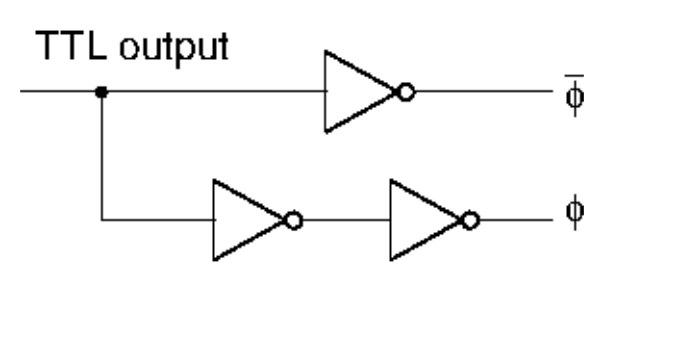
\includegraphics[width=70mm]{reports/lab6/TTL.png}
                \caption{Circuit diagram of Switch Driving Circuit}
            \end{subfigure}%
            \begin{subfigure}{.5\textwidth}
                \centering
                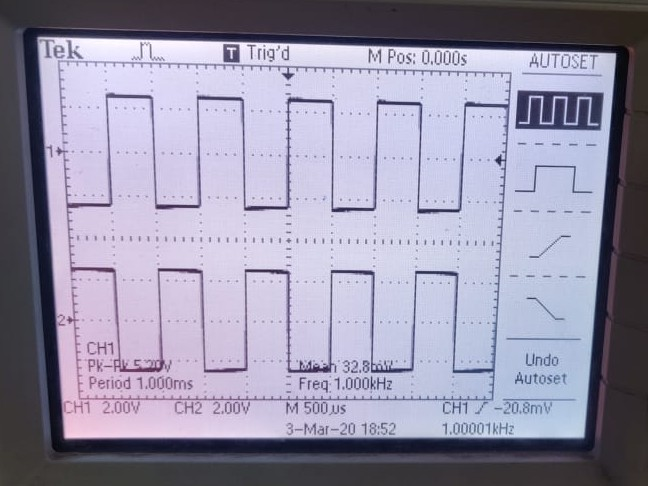
\includegraphics[width=70mm]{reports/lab6/phinphibar.jpeg}
                \caption{Output waveform of \phi and \(\bar \phi\)}
            \end{subfigure}%
        \end{figure}
        \noindent
        $\ast$ From the waveforms above, we can verify that the two signals are 180$^{\circ}$ apart.
        
%%%%%%%%%%%%%%%%%%%%%%%%%%%%%%%%%%%%%%%%%%%%%%%%%%%%%%%%%%%%%%%%%%%%%%%%%%%%%%%%%%%%%%%%%%%%%%%%%%%%%    
    \subsection{Switch based PSD}
    
        The switch based phase sensitive detector is the heart of the lock-in-amplifier, we construct it using IC CD4066 which has 4 bilateral switches in it, each of which requires a controlling input which tells the switch when to switch on or off.
        \begin{figure}[H]
            \centering
            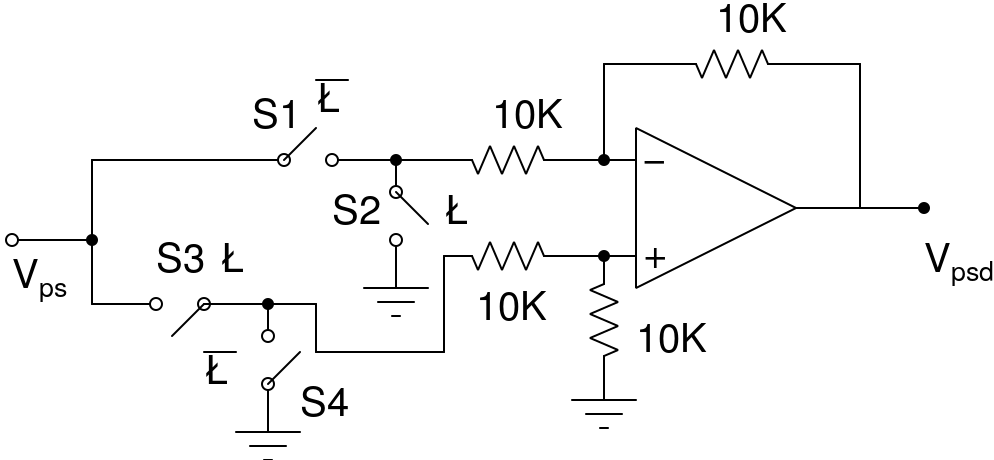
\includegraphics[width = 0.5\linewidth]{reports/lab6/psd.png}
            \caption{Circuit diagram of PSD}
        \end{figure}
        \noindent
        We use two complementary square wave signals \(\phi\) and \(\bar \phi\) as the control inputs. \(\phi\) is applied to \(S_2\) and \(S_3\), whereas \(\bar \phi\) is applied to \(S_1\) and \(S_4\) as shown above.\\\\
        Below are the waveforms obtained for various phase difference angles
        \begin{figure}[H]
            \centering
            \begin{subfigure}{.5\textwidth}
                \centering
                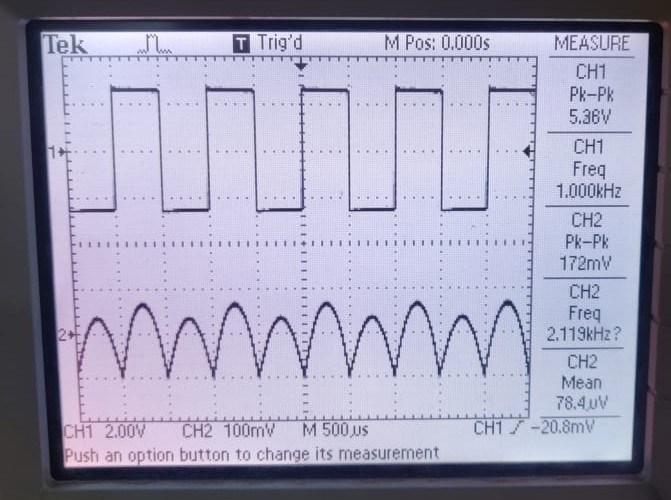
\includegraphics[width=70mm]{reports/lab6/0.jpeg}
                \caption{Output waveform for 0^{\circ}}
            \end{subfigure}%
            \begin{subfigure}{.5\textwidth}
                \centering
                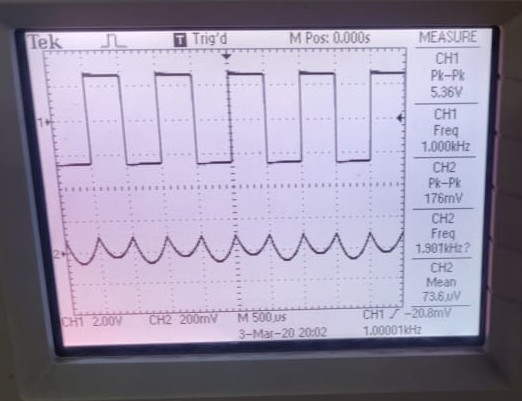
\includegraphics[width=70mm]{reports/lab6/180.jpeg}
                \caption{Output waveform for 180^{\circ}}
            \end{subfigure}%
        \end{figure}
        \begin{figure}[H]
            \centering
            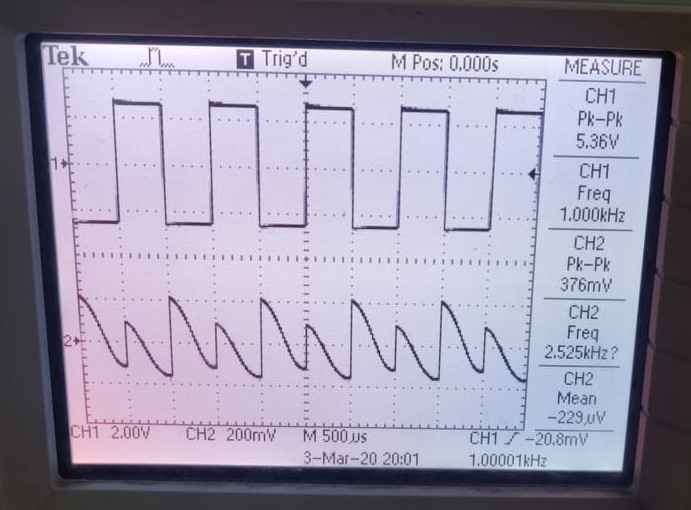
\includegraphics[width = 0.5\linewidth]{reports/lab6/minus90.jpeg}
            \caption{Output waveform for -90^{\circ}}
        \end{figure}
        \noindent
    
%%%%%%%%%%%%%%%%%%%%%%%%%%%%%%%%%%%%%%%%%%%%%%%%%%%%%%%%%%%%%%%%%%%%%%%%%%%%%%%%%%%%%%%%%%%%%%%%%%%%%%   
    \subsection{Low Pass Filter}
        The circuit connections of the low pass filter are shown in figure below:
        \begin{figure}[H]
            \centering
            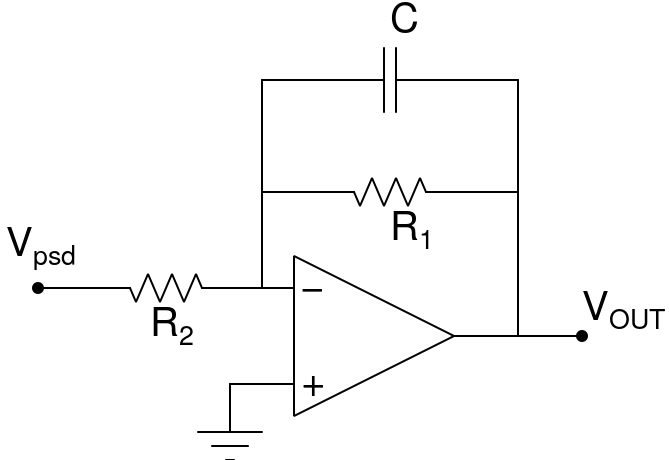
\includegraphics[width = 0.4\linewidth]{reports/lab6/LPF.png}
            \caption{Low Pass Filter}
        \end{figure}
        \noindent
        The output of the Phase Sensitive Detector consists of a DC component and high frequency components, we use the low pass filter to filter out the high frequency component and obtain the DC component.
        The transfer function of the Low Pass Filter is given by,
        \begin{equation}
            H(j\omega)=\frac{1}{1+j\omega \times 15k\Omega \times 1\mu F}=\frac{1}{1+j\omega \times 15ms}
        \end{equation}
        \noindent
        The phase response of the Low Pass Filter is given by,
        \begin{equation}
            \angle H(j\omega)=-\arctan(\omega \times 15k\Omega \times 1\mu F)=-\arctan(\omega \times 15ms)
        \end{equation}
        \noindent
        The magnitude response of the Low Pass Filter is given by,
        \begin{equation}
            |H(j\omega)|=\frac{1}{1+(\omega \times 15k\Omega \times 1\mu F)^2}=\frac{1}{1+(\omega \times 15ms)^2}
        \end{equation}
        \noindent
        We construct the circuit as shown above and test the circuit by applying a \(1V_{pp}\) input signal with frequency ranging from 1Hz to 1kHz to obtain its frequency response plot as shown below.
        
        \begin{center}
            \begin{tabular}{|c|c|c|}
            \hline
            Frequency(Hz)  &   \(|\)H(j\(\omega\))\(|\) &   \(A_v=20\log{H}\) (in dB) \\
            \hline
            1   &   1.8     &    5.105    \\
            2   &   0.976 &   -0.214    \\
            5   &   0.931 &   -0.621    \\
            10   &   0.893 &   -0.984    \\
            20      &   0.521 &   -5.666    \\
            50      &   0.225   &   -12.937    \\
            100    &   0.127 &   -17.893    \\
            200 &   0.067 &   -23.439    \\
            500    &   0.048 &   -26.361     \\
            1000 &   0.029 &   -30.798    \\
            \hline
            \end{tabular}
        \end{center}
        \begin{figure}[H]
            \centering
            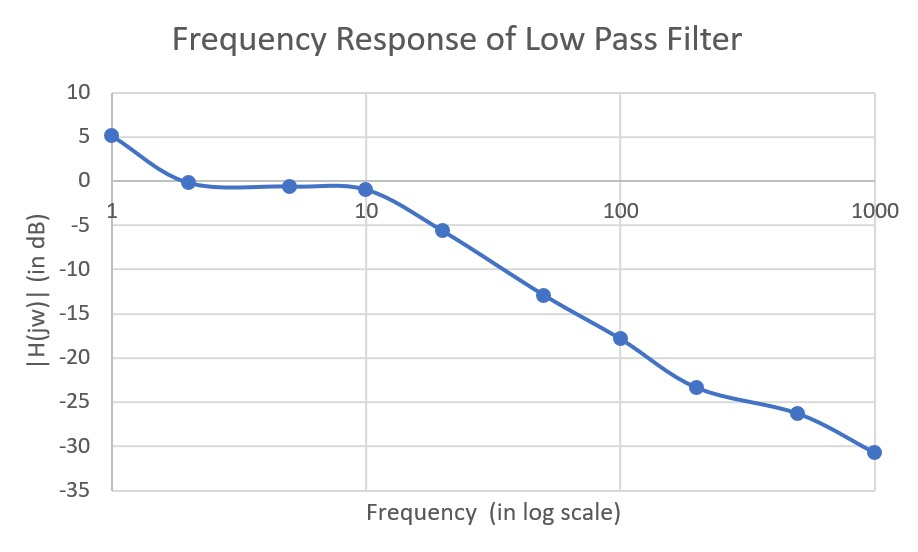
\includegraphics[width = 0.5\linewidth]{reports/lab6/response.jpeg}
            \caption{Magnitude response}
        \end{figure}
        \noindent
        The theoretical value of cut off frequency of the low pass filter is \textbf{10.61Hz}\\\\
        The output of the PSD(\(V_{psd}\)) is fed into the low pass filter, and the higher harmonics of \(V_{psd}\) are rejected to obtain a DC output, the results we obtained are tabulated below.\\\\
        \noindent
        The output of $V_{psd}$ is connected to the low pass filter which retains the DC component present in $V_{psd}$. Below are some of the output waveforms, obtained on passing through the low pass filter.
        % \begin{figure}[H]
        %     \centering
        %     \begin{subfigure}{.5\textwidth}
        %         \centering
        %         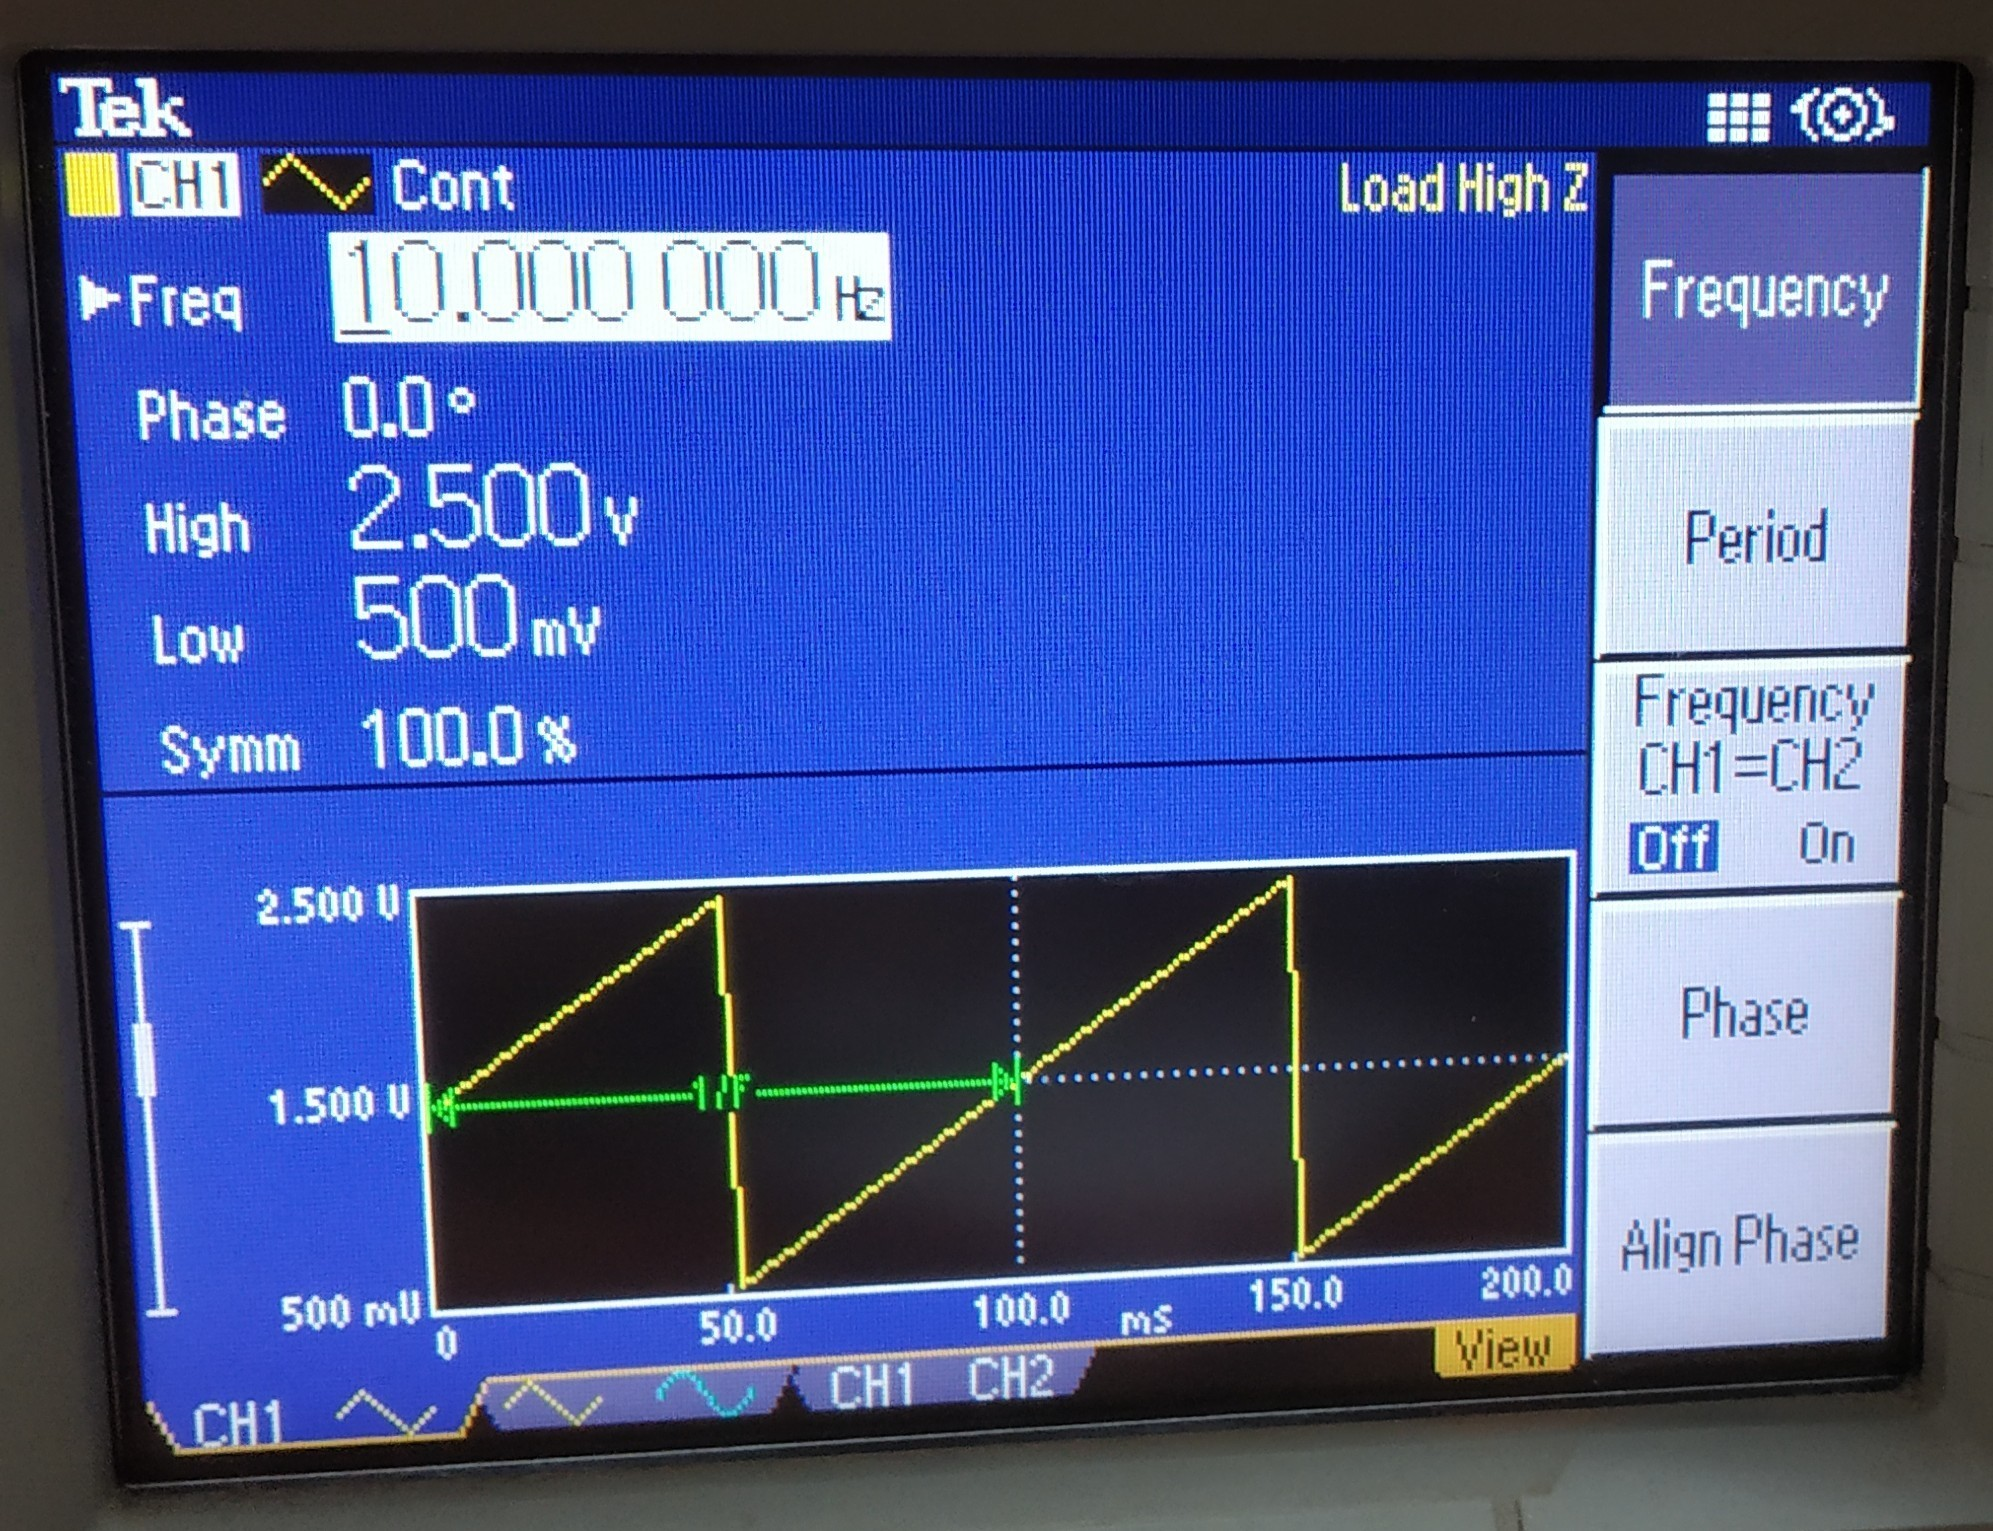
\includegraphics[width=70mm]{reports/lab5/ramp.jpg}
        %         \caption{Ramp signal}
        %     \end{subfigure}%
        %     \begin{subfigure}{.5\textwidth}
        %         \centering
        %         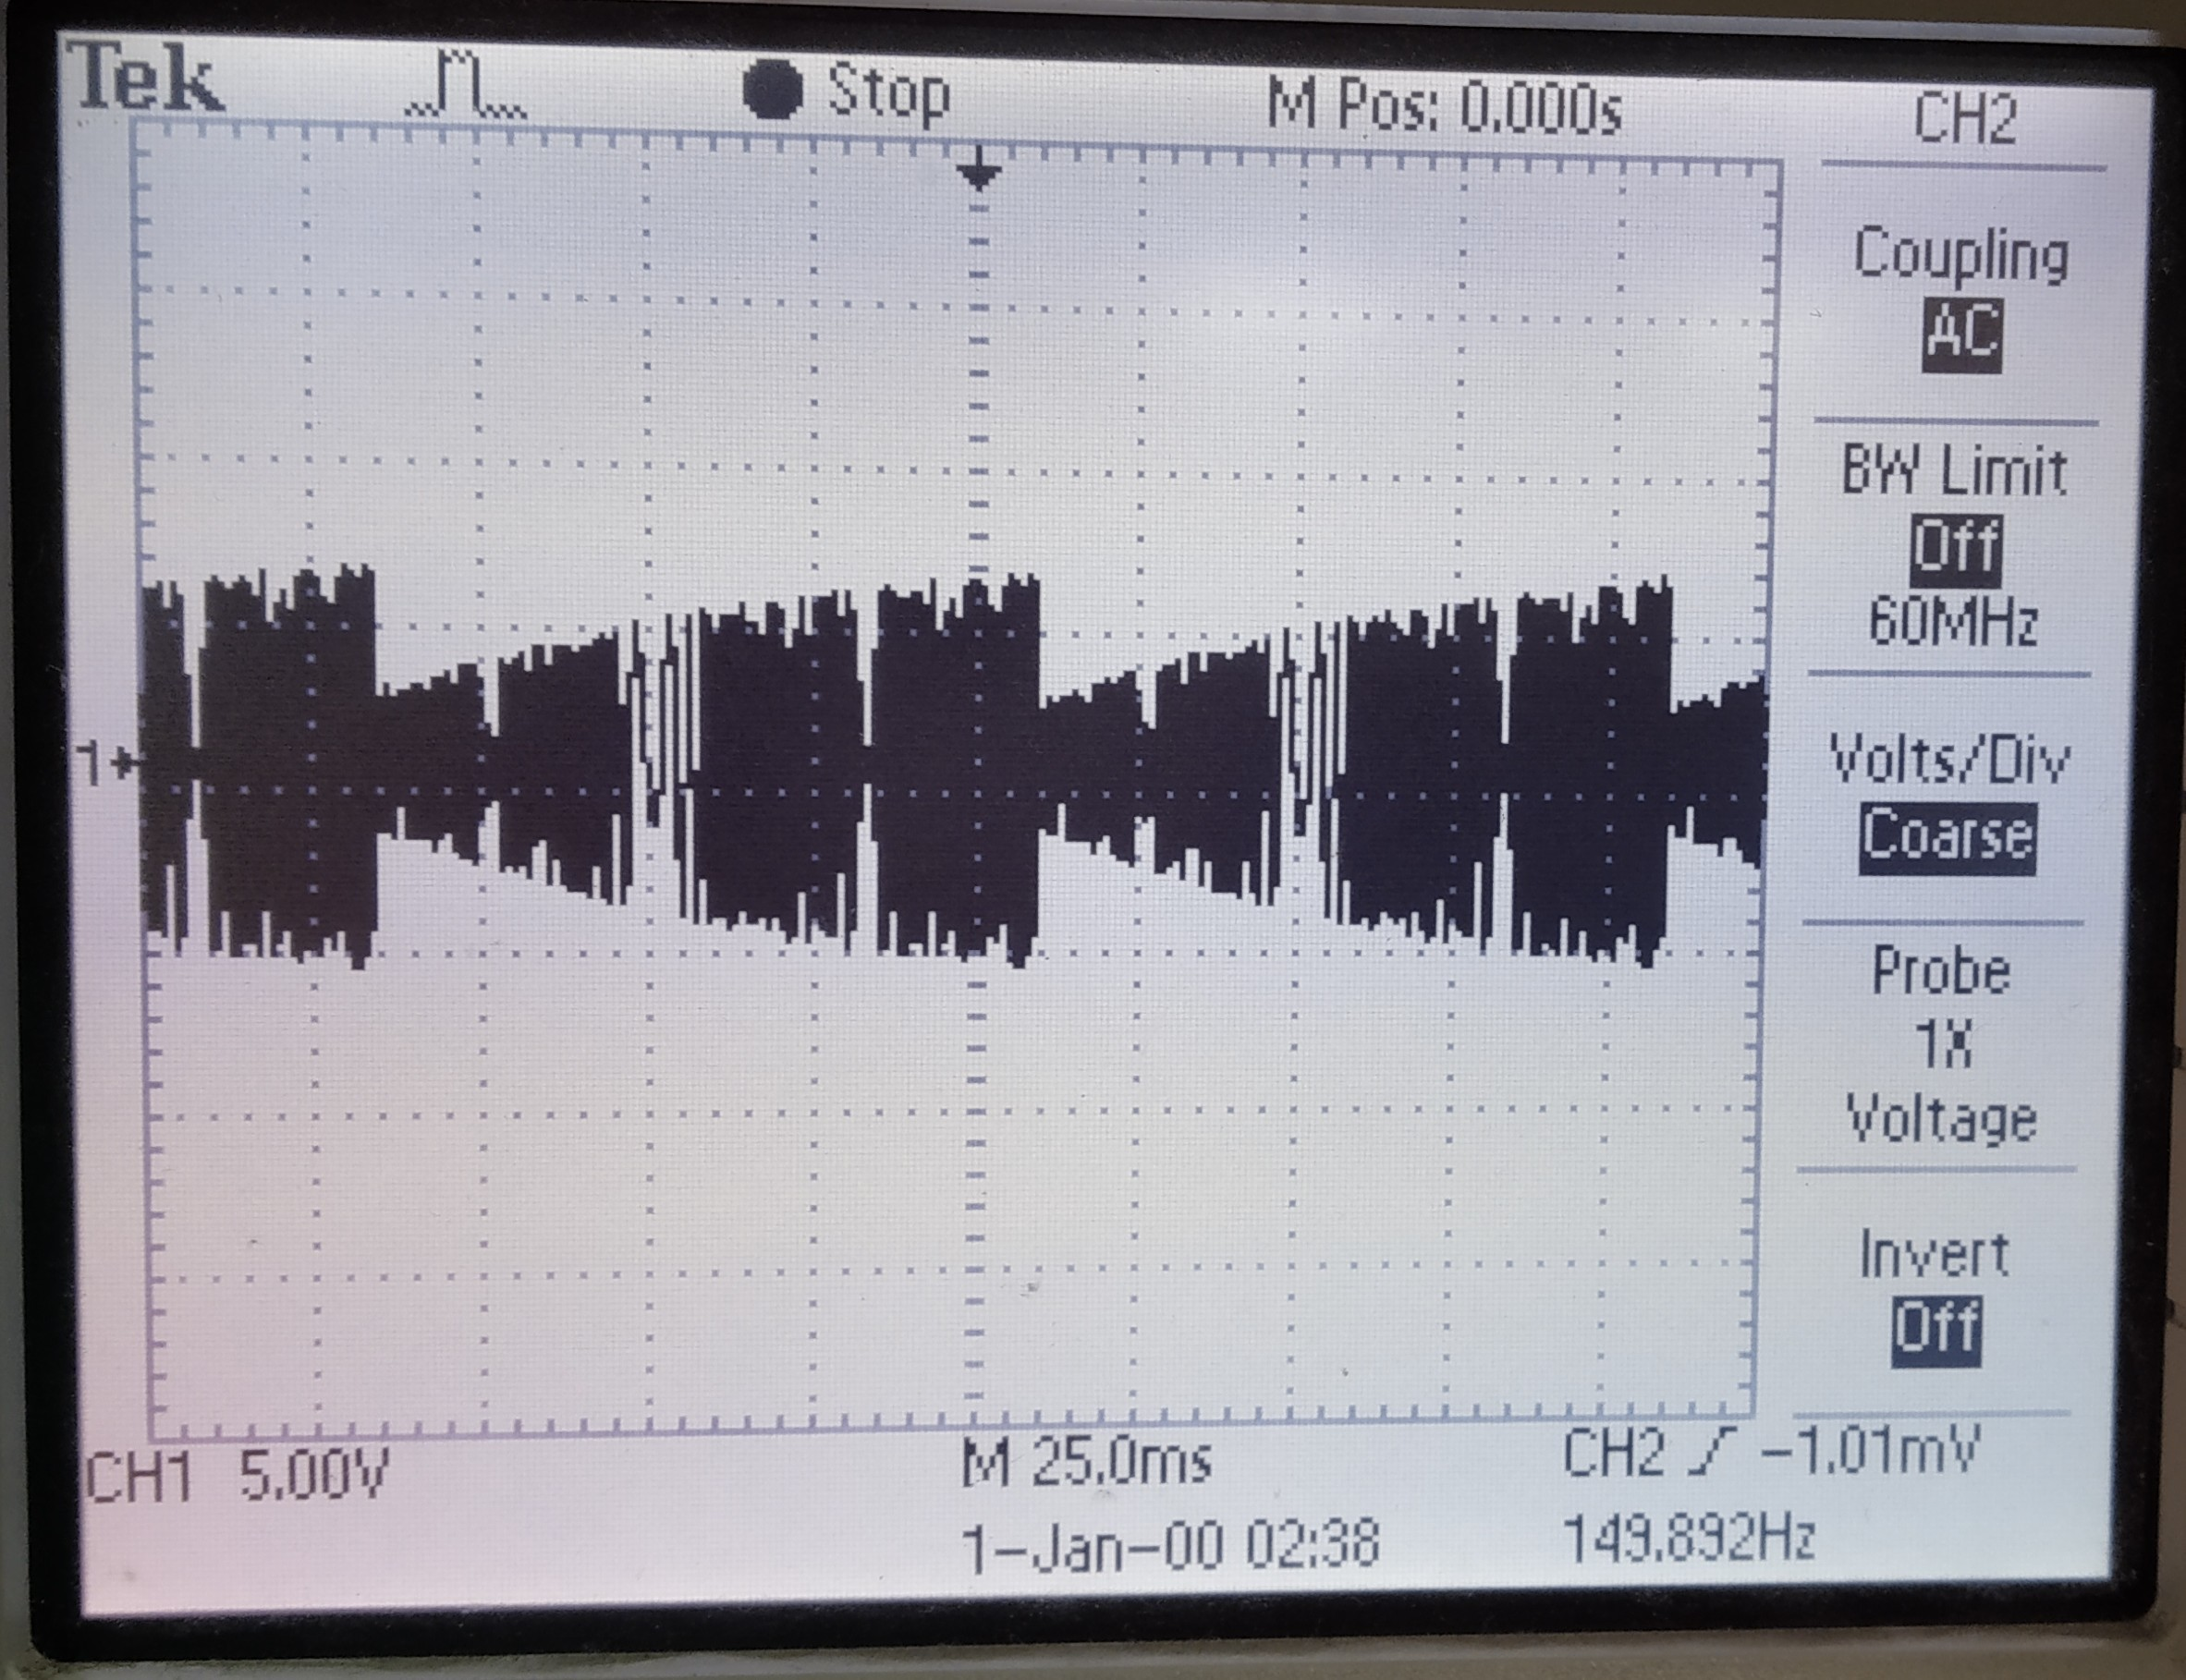
\includegraphics[width=70mm]{reports/lab5/highpassfilter.jpg}
        %         \caption{Frequency Response of ramp signal}
        %     \end{subfigure}%
        % \end{figure}
        % \begin{figure}[H]
        %     \centering
        %     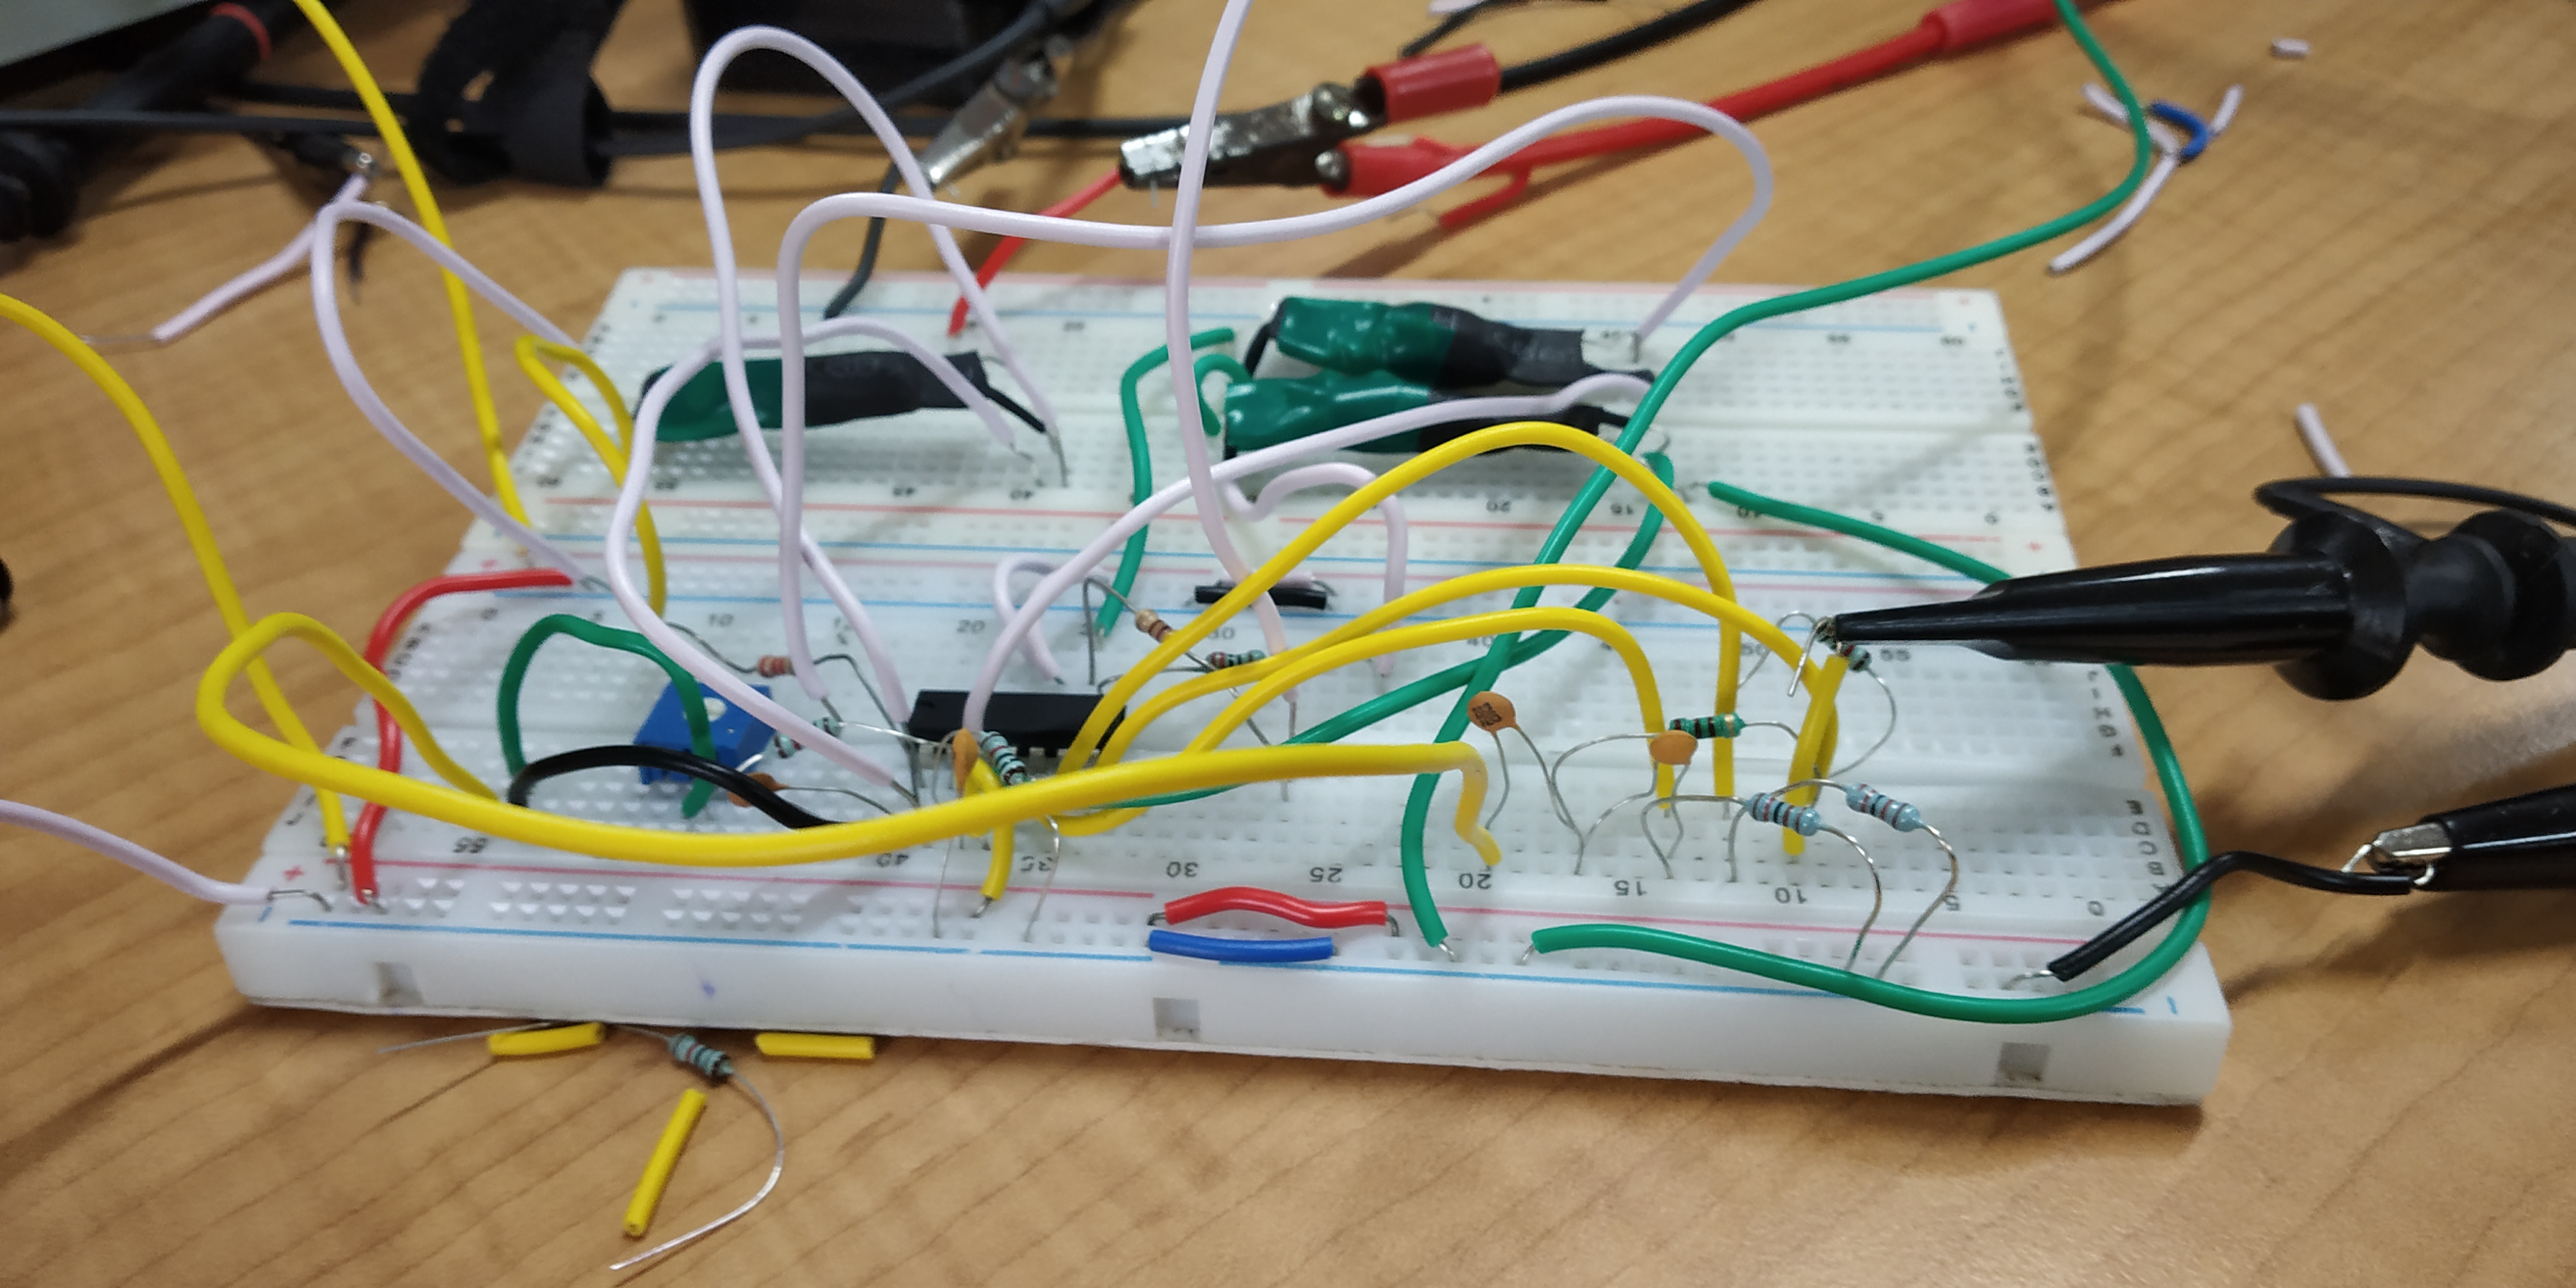
\includegraphics[width = 0.5\linewidth]{reports/lab5/inLab_ckt2.jpg}
        %     \caption{Bread-board circuit of Sweep generator with High Pass Filter}
        % \end{figure}
        The results are tabulated as follows:
        \begin{center}
        \begin{tabular}{|c|c|c|}
            \hline
            Phase Difference(^\circ)  &  Average of \(V_{psd}\) (mV) &   DC output of LPF (mV) \\
            \hline
            0   &    358   &    339    \\
            -90   &   -0.38 &   -0.14    \\
            -180   &   -261 &   -236    \\
            \hline
            \end{tabular}
        \end{center}
%%%%%%%%%%%%%%%%%%%%%%%%%%%%%%%%%%%%%%%%%%%%%%%%%%%%%%%%%%%%%%%%%%%%%%%%%%%%%%%%%%
\section{Conclusions}
\begin{itemize}
    \item We derived the transfer function of the Phase Shifter and found the values of resistances in the Phase Shifter at which we obtain phase differences of 0\(^\circ\), -45\(^\circ\), -90\(^\circ\), -135\(^\circ\), -180\(^\circ\) and we observe that these values close to the theoretical values of the same.
    \item We derived the transfer function of the Low Pass Filter and plotted its frequency response to find its cut off frequency to be 10Hz which is close to the theoretical value 10.61Hz.\\\\
    We found the average value of \(V_{psd}\) and the DC output obtained at the LPF to be nearly the same.
    \item We found the average value of $V_{psd}$ and the DC output obtained at the LPF to be nearly the same.
        \begin{center}
        \begin{tabular}{|c|c|c|}
            \hline
            Phase Difference(^\circ)  &  cos \phi &   Observed cos \phi \\
            \hline
            0   &    1   &    1.065    \\
            -90   &   0 &   -4.4 \times 10^{-4}    \\
            -180   &   -1 &   -0.74    \\
            \hline
            \end{tabular}
        \end{center}
        where Observed cos $\phi$ = $\frac{V_{out}}{\frac{2A}{\pi}}$\\\\
    \noindent
    For -180\(^\circ\), the cos $\phi$ doesn't match because the resistance value required is \infty.
\end{itemize}
    \\\\
    \noindent
    Thus, we analyzed a phase detection circuit which can calculate the phase difference between two input signals.

%%%%%%%%%%%%%%%%%%%%%%%%%%%%%%%%%%%%%%%%%%%%%%%%%%%%%%%%%%%%%%%%%%%%%%%%%%%%%%%%%%%
\vspace{4cm}

    \begin{thebibliography}{9}

        \bibitem{supporting doc} Experiment Handout
        \bibitem{} Teaching phase-sensitive demodulation for signal condition to undergraduate students, \textit{Wuqiang Yang}
        \bibitem{} Datasheet of IC CD4066
        
    \end{thebibliography}

\end{document}

%%%%%%%%%%%%%%%%%%%%%%%%%%%%%%%%%%%%%%%%%%%%%%%%%%%%%%%%%%%%%%%%%%%%%%%%%%%%%%%%%%%%%%%%%%%%%%%%%%%%%%%%%%%%%